%\documentclass{cumcmthesis}
\documentclass[withoutpreface,bwprint]{cumcmthesis} %去掉封面与编号页
\title{基于改进启发式算法和规划模型的传感器充电路线规划问题}
\tihao{A} % 题号
\baominghao{4321} % 报名号
\schoolname{湘潭大学}
\membera{米科润}
\memberb{周昕阳}
\memberc{李云潇}
\supervisor{杨柳}
\yearinput{2021} % 年
\monthinput{09} % 月
\dayinput{12} % 日
\bibliographystyle{plain}
%\usepackage[ruled,boxed,commentsnumbered]{algorithm2e}
\usepackage{algorithm,algpseudocode,float}
\usepackage{lipsum}
%\renewcommand{\algorithmcfname}{算法}
\usepackage{bm}

\makeatletter
\newenvironment{breakablealgorithm}
  {% \begin{breakablealgorithm}
   \begin{center}
     \refstepcounter{algorithm}% New algorithm
     \hrule height.8pt depth0pt \kern2pt% \@fs@pre for \@fs@ruled
     \renewcommand{\caption}[2][\relax]{% Make a new \caption
       {\raggedright\textbf{\ALG@name~\thealgorithm} ##2\par}%
       \ifx\relax##1\relax % #1 is \relax
         \addcontentsline{loa}{algorithm}{\protect\numberline{\thealgorithm}##2}%
       \else % #1 is not \relax
         \addcontentsline{loa}{algorithm}{\protect\numberline{\thealgorithm}##1}%
       \fi
       \kern2pt\hrule\kern2pt
     }
  }{% \end{breakablealgorithm}
     \kern2pt\hrule\relax% \@fs@post for \@fs@ruled
   \end{center}
  }
\makeatother

\begin{document}
\maketitle
\begin{abstract}
物联网正以惊人的方式改变着我们的世界。物与物之间进行无线通信,可以自动进行数据交换并大大提高效率,这对生活和生产产生了积极影响。物联网的基础是传感器技术,新技术革命的到来,世界开始进入信息时代。在利用信息的过程中,首先要解决的就是要获取准确可靠的信息,而传感器是获取自然和生产领域中信息的主要途径与手段。本文针对无线可充电传感器网络充电路线规划进行研究,基于数学规划方法和启发式算法,分别给出系统在单个移动充电器MC(Mobile Chager)和四个移动充电器的情况下,相应的最佳线路规划以及各传感器(Seneors)的最低电池容量。\par
关于问题一,由于仅需考虑移动充电器在充电路途上的能量消耗,故我们将此问题转化为求解TSP的最短哈密顿回路问题。对附件1的数据进行处理,得出任意两点之间的路径长度,在此基础上为求解此NP难问题。首先,为了提高速率以适应现实情况,我们采用改进的模拟退火算法和遗传算法,得出近似最优化的路径。而为求得精确的最短路径,我们运用0-1整数规划的方法,在Matlab使用Gurobi进行加速计算,得出精确最优路径,其路径长度为11.4832km,经对照,该精确解与启发式算法求出的精确解极为接近,这从一定程度上反映了改进后启发式算法的优势。\par
关于问题二,基于问题一的模型中由整数规划得出的最优路径,查询相关资料后我们对参数进行合理的假设。伴随证明,我们给出了简化模型的定理,在定理的保证下,我们讨论移动充电器每次为各传感器从最低电池容量充电至电池容量的情况,建立无线传感器系统维持稳定的非线性规划模型,使用Matlab对其进行求解,得出在保证整个系统一直正常运行的条件下,各传感器的电池的最低电池容量,对应的结果输出于表格,并且发现电池容量差异符合实际情况,于是得出结论:所建立模型表现良好。\par
关于问题三,基于问题一、二模型的基础上讨论四台移动充电车的耗电情况以及如何保持系统稳定,经过分析,我们将耗电问题转化为车辆路径(VRP)问题,并类似问题一建立新的规划模型,利用Matlab对其进行求解,路径结果在文中以图片形式给出,并且求得最短路径为12.8098(km),接下来,我们将所得路径代入问题二模型求得各传感器的最低电池容量,结果以表格展示,同时凭借容量差异得到模型表现良好的结论。


\keywords{启发式算法\quad 规划模型\quad TSP\quad VRP\quad}
\end{abstract}



\section{问题重述}
\subsection{问题背景}
随着物联网的快速发展,无线传感器网络WSN在生活中的应用越来越广泛。一个无线传感器网络包括一些传感器和一个数据中心。传感器从环境中收集信息,并定期将收集的信息发送到数据中心。数据中心对数据进行分析并发回控制信息。\par
影响WSN生命周期的最重要因素之一是能源。为了使WSN能够连续运行,它必须不断地提供能源。提供能量的一种方式是通过能量采集,它允许传感器从环境中吸取自己的能量,通过使用环境能源如太阳能或风能来维持其运行。但是,这种方式提供的能量不仅不稳定,而且过于依赖环境,一旦环境不满足条件,WSN无法从环境中吸取能量自然也就无法运行。另一种提供能量的方式是电池供电,移动充电器定期补充传感器的电池,从而为WSN的运行提供源源不断的能量。以这种方式供电的网络也被称为无线可充电传感器网络。\par



\subsection{问题的提出}
一个无线充电传感器网络由三个部分组成:一个数据中心DC,几个传感器,以及一个或多个移动充电器MC。\par
数据中心和几个传感器分布在一个二维空间中,如下\ref{fig:simple}所示(虚线箭头表示数据中心和传感器之间,以及传感器和传感器之间的路径;实线箭头表示MC的充电路线)。\par
\begin{figure}[!h]
    \centering
    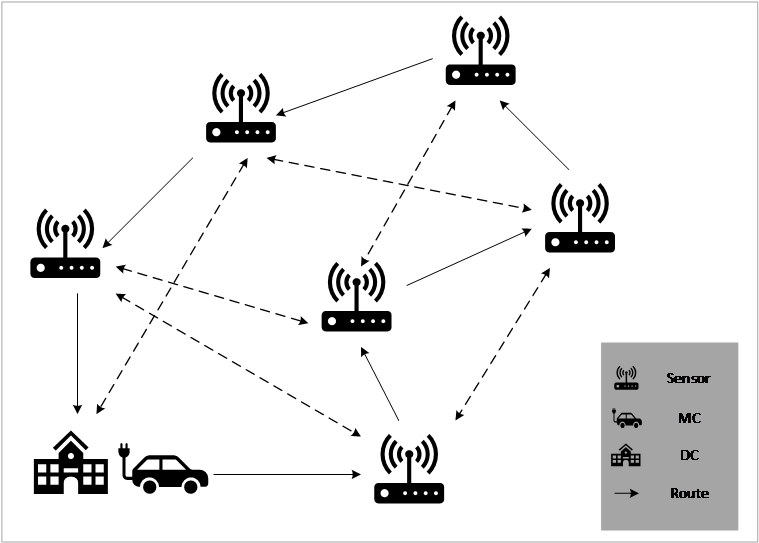
\includegraphics[width=.6\textwidth]{C001}
    \caption{问题简图}
    \label{fig:simple}
\end{figure}
在这个系统中,传感器从环境中收集信息,并将收集的信息传输到数据中心。为了使WRSN正常运行,移动充电器需要定期为传感器充电,以防止它们低于阈值水平。移动充电器从数据中心出发,以固定的速度依次经过每个传感器,在每个传感器上停留一段时间,并以恒定的充电速率为传感器充电,直到所有的传感器都充电完毕,再返回数据中心。每个传感器都有其特定的能量消耗速率,和一个固定的电池容量。移动充电器的能量消耗主要体现在两个方面:一是为传感器节点充电引起的正常能量消耗,二是移动充电器在为传感器充电途中的能量消耗。为了减少移动充电器在路上的能量消耗,需要对移动充电器的充电路线进行合理规划。考虑以下问题:
\begin{enumerate}[itemsep=0pt,parsep=0pt,label=(\arabic*)]
\item 给出每个节点的经纬度,考虑在只派出一个移动充电器的情况下,如何规划移动充电器的充电路线,使移动充电器在路上的能量消耗最小。
\item 如果给定每个节点的经纬度,每个节点的能量消耗率,并假定传感器的功率只有在高于$f(mA)$时才能正常工作,移动充电器的移动速度为$v(m/s)$,移动充电器的充电速度为$r(mA/s)$,在只派出一个移动充电器的情况下,如果采用问题1中规划的充电路线,求解每个传感器的电池容量至少应该是多少,以保证整个系统一直正常工作(即系统中每个传感器的电量不会低于$f(mA)$)。
\item 若给出每个节点的经纬度、每个节点的能量消耗速率,并假设传感器的电量只有在高于$f(mA)$时才能正常工作,移动充电器的移动速度为$v(m/s)$、移动充电器的充电速率为$r(mA/s)$,为了提高充电效率,同时派出4个移动充电器进行充电,求解应如何规划移动充电器的充电路线使所有移动充电器在路上的总能量消耗最小,求解每个传感器的电池的容量应至少多大才能保证整个系统一直正常运行。
\end{enumerate}





\section{问题分析}
针对问题一,题目在给出无线充电传感器网络中数据中心和各传感器位置后,要求制定移动充电器的充电路线使得移动充电器在路上的能量消耗最小。考虑到移动充电器行进时间越长或者说行进里程越大,其在路上消耗的能量越多,于是此问题转换为TSP问题,即求解当移动充电器从数据中心出发遍历每一传感器后回到数据中心的最短路径。本文将对此问题运用启发式算法求解近似解以及运用0-1整数规划方法求取精确解。\par
针对问题二,题目要求我们采用问题一规划出来的充电线路,求解保证整个系统一直正常运行的每个传感器的电池最大容量。由于题目所提供参数:移动充电器的移动速度、移动充电器的充电速率、传感器最低电池容量均为未知,而本文所要建立的非线性规划模型需要明确这些参数的值,于是我们将经过查询资料和相关文献假定参数的值并代入模型求解,同时对第一圈充电和一般情况充电进行进一步讨论,最后对模型进行稳定性分析。\par
针对问题三,题目要求我们解决当同时派出四台移动充电车时,规划移动充电器的充电路线以最小化所有移动充电器在路上总的能量消耗并且求解每个传感器的电池的容量应至少是多大才能保证整个系统一直正常运行。显然,这要求我们解决一个车辆规划(VRP)问题,我们将类似问题一建立整数规划模型,并利用问题二建立的模型解决电池的最大容量问题。











	\section{模型的假设}
	\begin{itemize}
	\item 移动充电器在回到数据中心后,瞬间更新自身能量,不做停顿,立即从数据中心出发为传感器节点充电;
	\item 不考虑障碍物的影响;
	\item 所有传感器的结构性能均相同,且不考虑设备的损耗;
	\item 任何情况下,移动充电器均能从数据中心出发,为所有传感器充电之后返回数据中心。
	\end{itemize}\par	
	
	
	
	
	

	\section{符号说明}
	\begin{center}
		%\centering
		\label{tabfuhao}
		\renewcommand{\arraystretch}{2}%调行距
		\setlength\tabcolsep{15pt}%设置列间距
		\begin{longtable}{cccc}
		\toprule[1.5pt]
		符号 & 说明 \\
		\midrule[1pt]
	$f$ & 传感器运行最低电量   \\
	$v$ & 移动充电器的移动速度\\
	$r$ & 移动充电器的充电效率    \\
	$u_1,u_{33}$ & 数据中心\\
	$u_i$ & 传感器 \\
	$z$ & 移动充电器行驶距离 \\
	$n$ & 传感器个数    \\
	$d_{ij}$ & 传感器i与传感器j之间的距离\\
	$c_i$ & 传感器最大电池容量   \\
	$N$ & 传感器集合 \\
	$A$ & 路径集合  \\
	$K$ & 移动充电器集合 \\
	$T$ & 单个充电周期总时长  \\
	$M$ & 极大实数(10000)\\
		\bottomrule[1.5pt]
		\end{longtable}
	\end{center}

	




	











\section{问题一:关于移动充电器的TSP模型}
由于本题只考虑移动充电器在充电路途中的能量消耗,并且移动充电器的能量消耗显然与路程长度呈正相关关系,我们遂将此问题转化为求解TSP的最短哈密顿回路问题。\par
TSP(旅行商问题)是这样一个问题:给定一系列城市和每对城市之间的距离,求解访问每一座城市一次并回到起始城市的最短回路,它是组合优化中的一个NP困难问题,因为NP困难问题未必可以在多项式时间内验证一个解的正确性\upcite{NPKunNan},但是对于充电路径规划等实际应用来说,需要在多项式时间内快速求得问题的解,因此采用启发式算法求解是十分必要的\upcite{无线可充电传感器网络充电规划方法研究}。
\subsection{启发式算法的模型建立与求解}
\subsubsection{改进的模拟退火算法}
模拟退火算法。最早的思想由Metropolis在1953年提出。KIRKPATRICK 等在1983年成功地应用在组合优化问题中,其出发点是基于物理中固体物质的退火过程与一般组合优化问题之间的相似性。在对固体物质进行退火处理时,常先将它加温使其粒子可以自由运动,然后使粒子系统的温度以足够慢的速度下降。若温度下降的速率足够慢,系统近似处于热力学平衡点。随着温度逐渐下降,最后系统将达到本身的最低能量状态,即基态,这相当于能量函数的全局最小点。组合优化问题的目标函数与能量等价,解与微观状态等价,最优解与能量最低状态等价。它是在一个给定温度下,搜索从一个状态随机变化到另一个状态,并用一个随机接受准则(Metropolis准则)进行判断。\par
与具有陷入局部最小值的缺点的基于梯度的gradient-based方法以及其他确定性搜索方法不同,模拟退火的主要优势在于其具有避免陷入局部最小值的能力。事实上,已经证明,如果足够的随机性与非常缓慢的冷却结合使用,模拟退火将收敛到其全局最优性。实质上,SA 是一种搜索算法,可以视为马尔可夫链,能够在合适的条件下收敛。这相当于将一些弹跳球放在某种景观上,当球弹跳并失去能量时,它们会稳定在某个局部最小点。如果球能够反弹足够长的时间且足够慢地失去能量,那么一些球将最终落入全局最低的位置,因此可以达到全局最小值\upcite{YANG201467}。\par
本文对模拟退火算法进行改进后的设计如下,流程图见其右:\\
\begin{minipage}[htbp]{0.65\linewidth}
\paragraph{Step 1}设定解空间$S(S$是将数据中心以1、31指代(表示起点和终点)而其他传感器以$2\ldots30$指代后的数值排列集合:$u_1\ldots u_{31}$)并且利用蒙特卡罗方法生成一个初始解$S_0$,同时令$T=T_0$,即开始退火的初始温度。
\paragraph{Step 2}设定目标函数$min f(S_i)=\sum_{i=1}^{31} d_{u_iu_{i+1}}$,$d_{ij}$为某两地距离
\paragraph{Step 3}根据当前解$S_i$,利用轮盘赌方法根据一定概率选择交换、逆转、插入方法进行扰动(这里设为0.2、0.3、0.5),产生一个新解$S_j$并计算相应的目标函数值$f(S_j)$,得到$\Delta f=f(S_j)-f(S_i)$。
\paragraph{Step 4}若$\Delta f<0$,则新解$S_j$被接受,作为新的当前解;若$\Delta f>0$,则新解$S_j$按概率$e^{\frac{-\Delta f}{T}}$被接受,T为当前温度。
\paragraph{Step 5}在温度T下,重复L次(L为Markov链长度,使得在每个T上达到准平衡)的扰动和接受过程,即执行步骤3与4。
\paragraph{Step 6}判断T是否已到达$T_{end}$,若是则终止算法得到最终行驶路径;否则降温后以新T继续计算。
\end{minipage}
\qquad
\begin{minipage}[htbp]{0.35\linewidth}
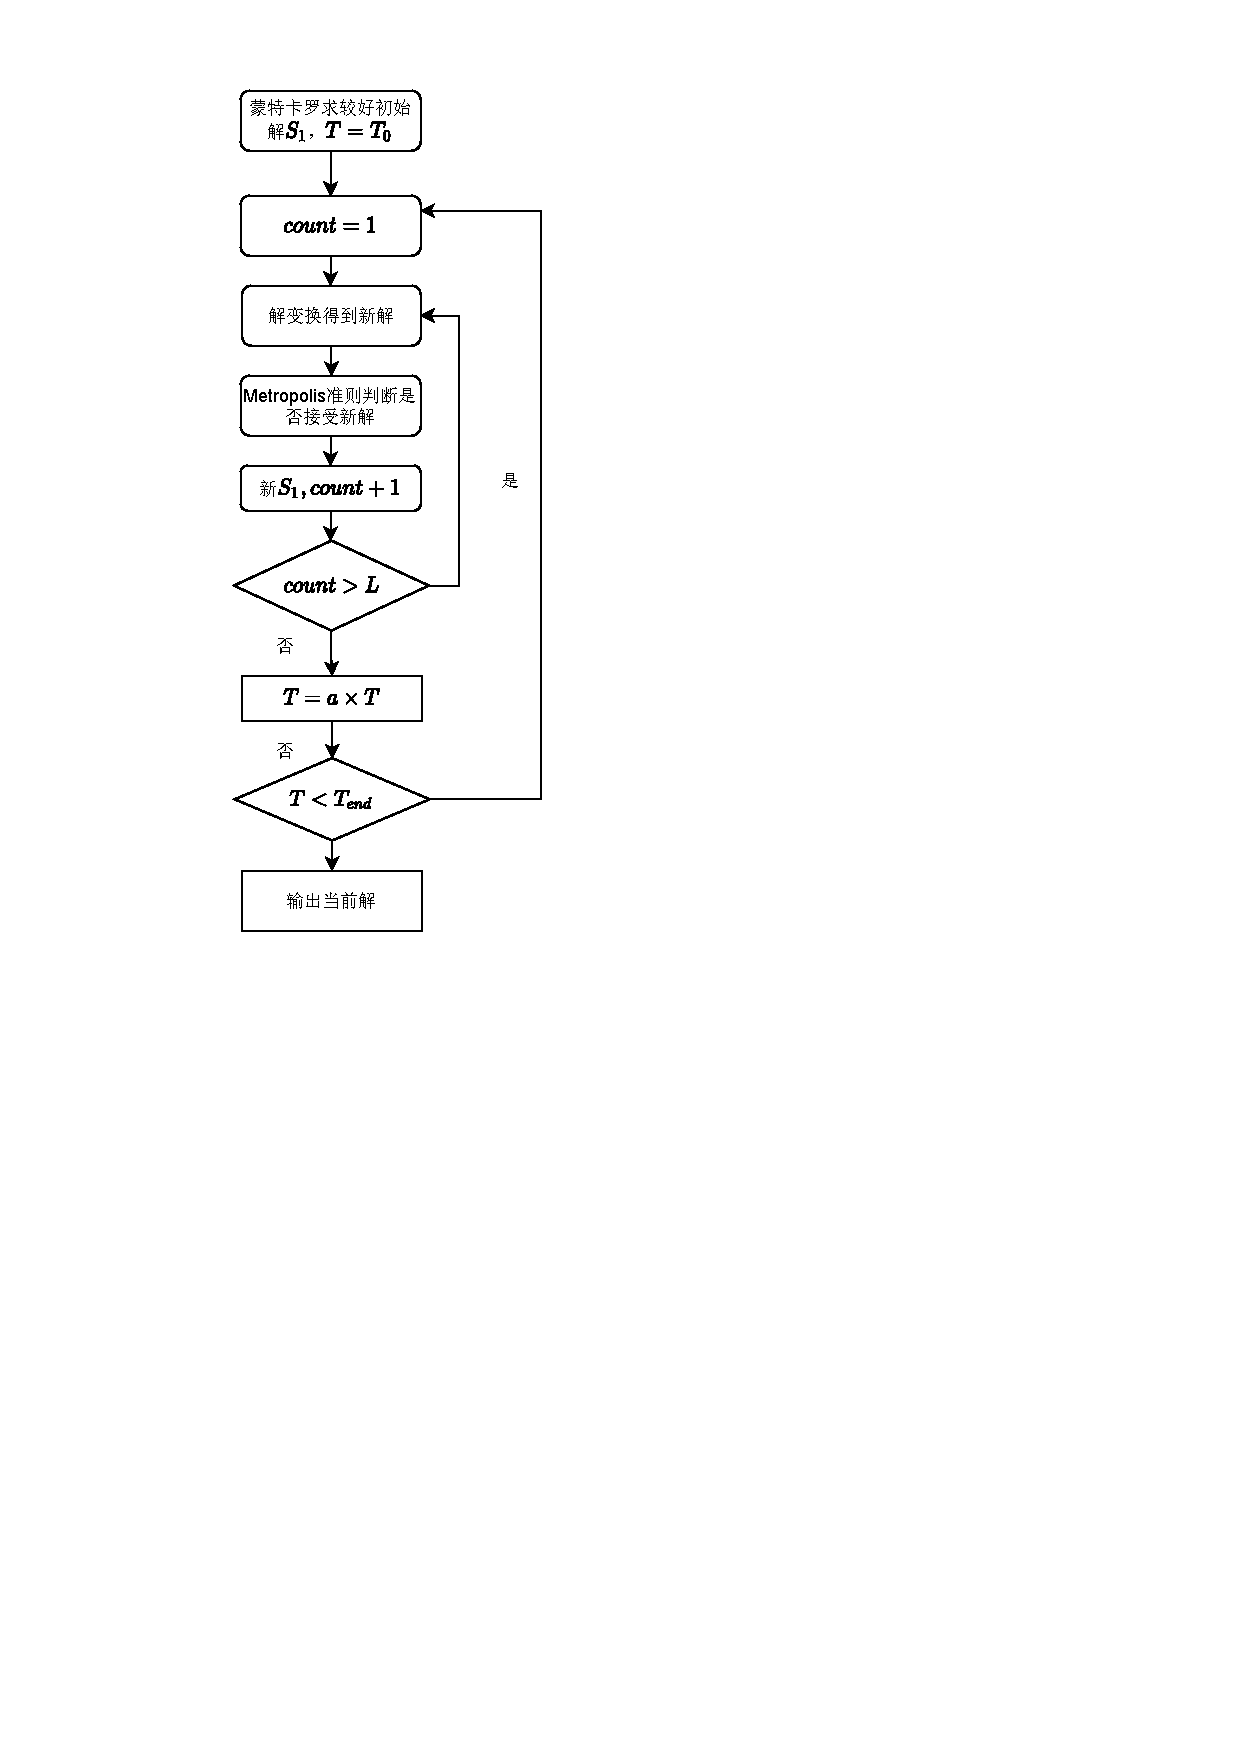
\includegraphics[height=18\baselineskip]{SA.pdf}
\end{minipage}\par



\subsubsection{改进的遗传算法}
遗传算法(Genetic Algorithms,GA)是一种基于自然选择原理和自然遗传机制的搜索(寻优)算法,它是模拟自然界中的生命进化机制,在人工系统中实现特定目标的优化。遗传算法的实质是通过群体搜索技术,根据适者生存的原则逐代进化,最终得到最优解或准最优解。它必须做以下操作:初始群体的产生、求每一个体的适应度、根据适者生存的原则选择优良个体、被选出的优良个体两两配对,通过随机交叉其染色体的基因并随机变异某些染色体的基因生成下一代群体,按此方法使群体逐代进化,直到满足进化终止条件\upcite{数学建模算法与应用}。\par
在遗传算法里,优化问题的解被称为个体,它表示为一个变量序列,称为染色体。染色体一般被表达为简单的字符串或数字符串,这一过程称为编码;首先,算法随机生成一定数量的个体,在每一代中,都会评价每一个体,并通过计算适应度函数(一般为目标函数)得到适应度数值。按照适应度排序种群个体,适应度高的排序靠前;确定进化参数群体规模、交叉概率、变异概率、进化终止条件后进行运算。\par
但是,遗传算法中适应函数的制定,人口规模的使用,突变和交叉率等重要参数的选择以及新群体的选择标准应当小心执行。任何不恰当的选择都会使算法难以收敛,产生无意义的结果。基于此,我们对遗传算法进行如下改进\upcite{数学建模算法与应用}:\par
\begin{itemize}
\item 将变异操作从交叉操作中分离出来,使其成为独立的寻优操作;
\item 采用“门当户对”式交叉:将父代个体按照适应度函数值进行排序,适应度值小的与小的配对,适应度大的与大的配对。然后利用混沌序列确定交叉点的位置,对确定的交叉项进行强度最弱的单点交叉;
\item 随机地取两个在2到30(代表29个传感器)之间的整数,对这两个数对应位置的基因附近进行较大强度的多个基因变异,变异时利用混沌序列把这两个位置的基因换成新的基因值,从而得到新的染色体;
\item 每次交叉和变异后,将排序在前百分之30的种群依次进行模拟退火操作,与原种群比较后提取较优的基因进入下次迭代。
\end{itemize}
上述遗传算法伪代码见算法1。\par

\begin{breakablealgorithm}
\caption{改进的遗传算法}
\begin{algorithmic}[1] %每行显示行号
  \State 适应度函数:$min f(\bm{u})=\sum_{i=1}^{31} d_{u_iu_{i+1}},\bm{u}=(u_1\ldots u_{31})$,$d_{ij}$为某两地距离;\\
  利用改良圈算法确定\textbf{初始解集};\\
  将初始解集编码为染色体(字符串);\\
  初始化交叉和变异的概率;\\

  \While{t < 最大进化代数}
    \State $\text{通过交配(从父代种群选择)、交叉和变异获得新的解集;}$
    \If{$\text{新解集有使总路径减小的解}$}
    \State $\text{将这些解预提取出来记作}J$
    \EndIf
	\While{g < J的数量的30\%}
		将第g个解进行模拟退火操作
		\If{模拟退火后g的适应度小于模拟退火前}
		\State 将原来的这个解替换
		\EndIf
		\State 更新 g=g+1   
		\State 更新 t=t+1
	\EndWhile
   \EndWhile
\end{algorithmic}
  %
\end{breakablealgorithm}


\subsubsection{结果分析}
针对问题运用Matlab实现改进的模拟退火、遗传算法。在改进的模拟退火算法中,蒙特卡罗迭代1000次,初始温度为100度,最低温为1度,温度衰减率为0.99,Markov链长度为10000,交换结构、交叉结构、插入结构的概率分别为0.2、0.3、0.5,最终路径长度结果为11.4832(km);在改进的遗传算法中,种群的个数为50,进化的代数为29次,最终路径长度结果为11.4832(km),优化过程见图\ref{fig:SAGA}

优化过程如图\ref{fig:SAGA}
\begin{figure}[!h]
    \centering
    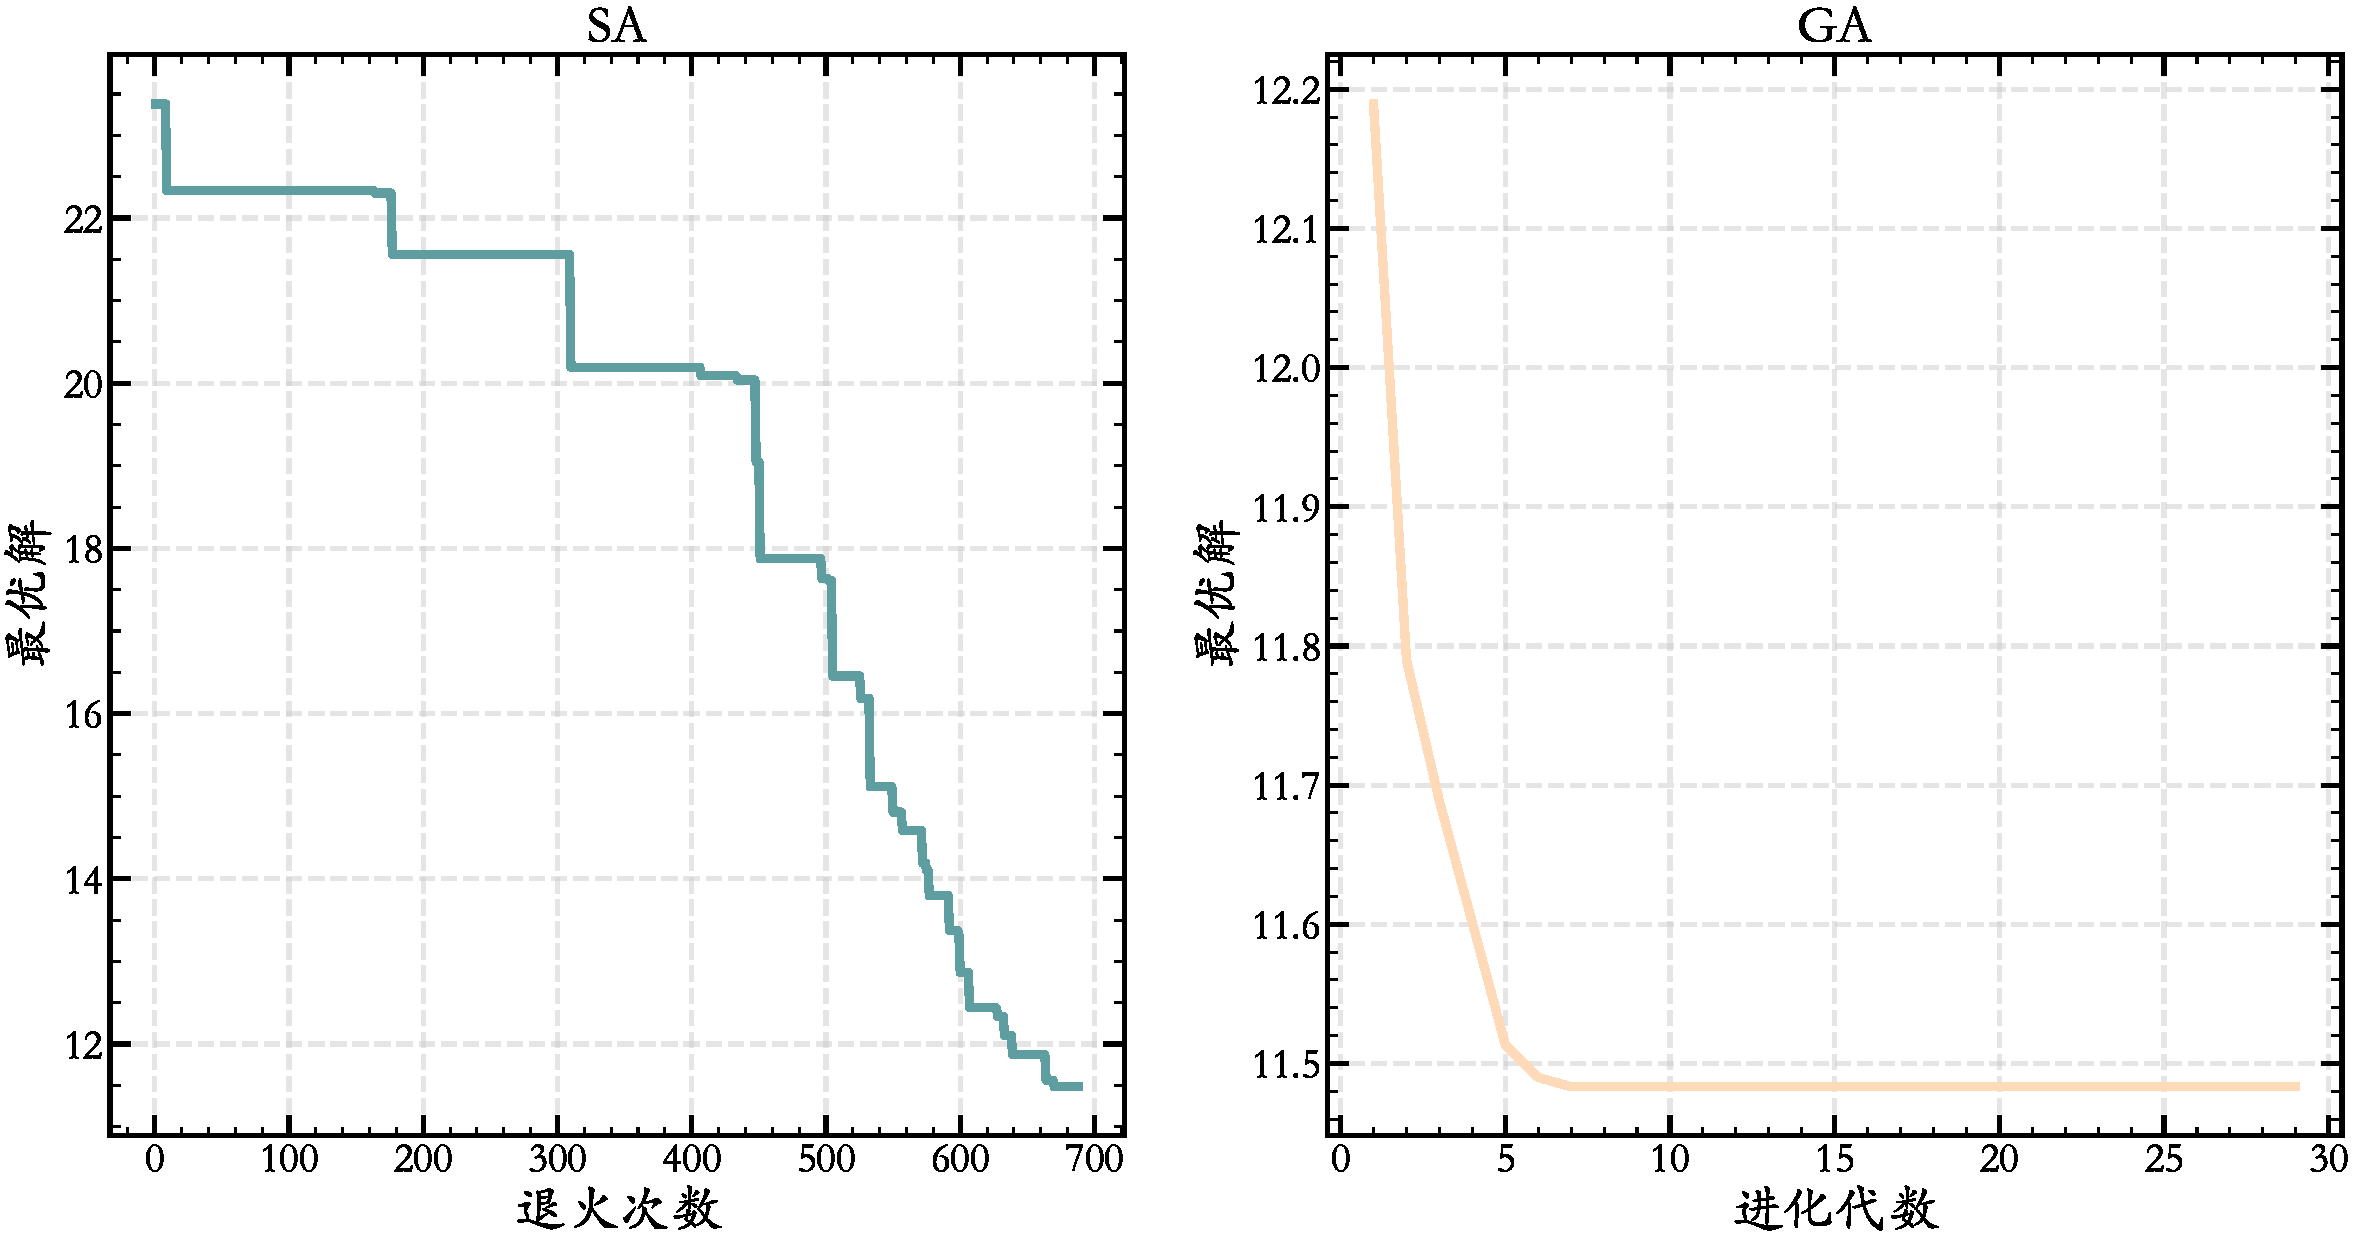
\includegraphics[width=1\textwidth]{SAGA}
    \caption{启发式算法优化过程}
    \label{fig:SAGA}
\end{figure}








\subsection{0-1整数规划模型的建立与求解}
为了对问题进行更科学的研究分析,除了上述启发式算法以外,针对对此题我们还建立了0-1整数规划模型,并在Matlab基础上通过接口使用线性规划求解器Gurobi在非常可观的时间内求出精确解。
\subsection{模型的建立}
\paragraph{决策变量 }将数据中心设为$u_1,u_{31}$(表示起点和终点),$u_2,\ldots,u_{30}$表示29个传感器,对任意两个地点$u_i,u_j$,定义变量$x_{ij}$来表示是否要从$u_i$出发访问$u_j$,定义变量$d_{ij}$表示$u_i,u_j$之间的距离,令
$$
x_{i j}=\left\{\begin{array}{l}
1 ,\text{如果移动充电器决定从}u_i\text{直接进入}u_j\\
0 ,\text{否则}\\
\end{array}\right.\\
$$
其中$i,j=1,2,\ldots,31$。
\paragraph{目标函数 }若移动充电器决定从$u_i\text{直接进入}u_j$,由已知,其行驶路程可表示为:
$$
z=\sum_{i=1}^{31} \sum_{j=1}^{31} d_{i j} x_{i j}
$$
其中,若$i=j\text{,则规定}c_{ii}=M\text{即一个充分大实数,}i,j=1,2,\ldots,31$
\paragraph{约束条件}
\begin{enumerate}
\item 每个传感器(或者是数据中心)恰好经过一次:
$$\sum_{i=1}^{31} x_{i j}=1, \quad j=1,2, \cdots, 31$$
\item 每个传感器(或者是数据中心)离开一次:
$$\sum_{j=1}^{31} x_{i j}=1, \quad i=1,2, \cdots, 31$$
\item 为防止在遍历过程中,出现子回路,即无法返回出发点的情形,附加一个强制性约束:
$$u_{i}-u_{j}+n x_{i j} \leq 30\quad i=1, \cdots, 31, j=2, \cdots, 31$$
其中$u_1=1,u_{31}=31$,$2\leq u_i\leq 30\quad i=2,\cdots,30$
\end{enumerate}\par

建立移动充电器TSP问题的0-1整数规划模型:
\begin{gather}
\min z=\sum_{i=1}^{31} \sum_{j=1}^{31} d_{i j} x_{i j}\\
\begin{cases}
\sum_{i=1}^{31} x_{i j}=1, \quad j=1,2, \cdots, 31\\
\sum_{j=1}^{31} x_{i j}=1, \quad i=1,2, \cdots, 31\\
u_{i}-u_{j}+n x_{i j} \leq 30\quad i=1, \cdots, 31, j=2, \cdots, 31\\
u_1=1,u_{31}=31, \quad 2\leq u_i\leq 30\quad i=2,\cdots,30 \\
x_{i j}=0 \text { 或1, } \quad i, j=1,2, \cdots, 31 .
\end{cases}
\end{gather}
\subsection{模型的求解与结果分析}
编写Matlab调用求解器Gurobi可得到如图\ref{fig:road}所示最优路径,同时求得最短距离为11.4832km。
\begin{figure}[!h]
    \centering
    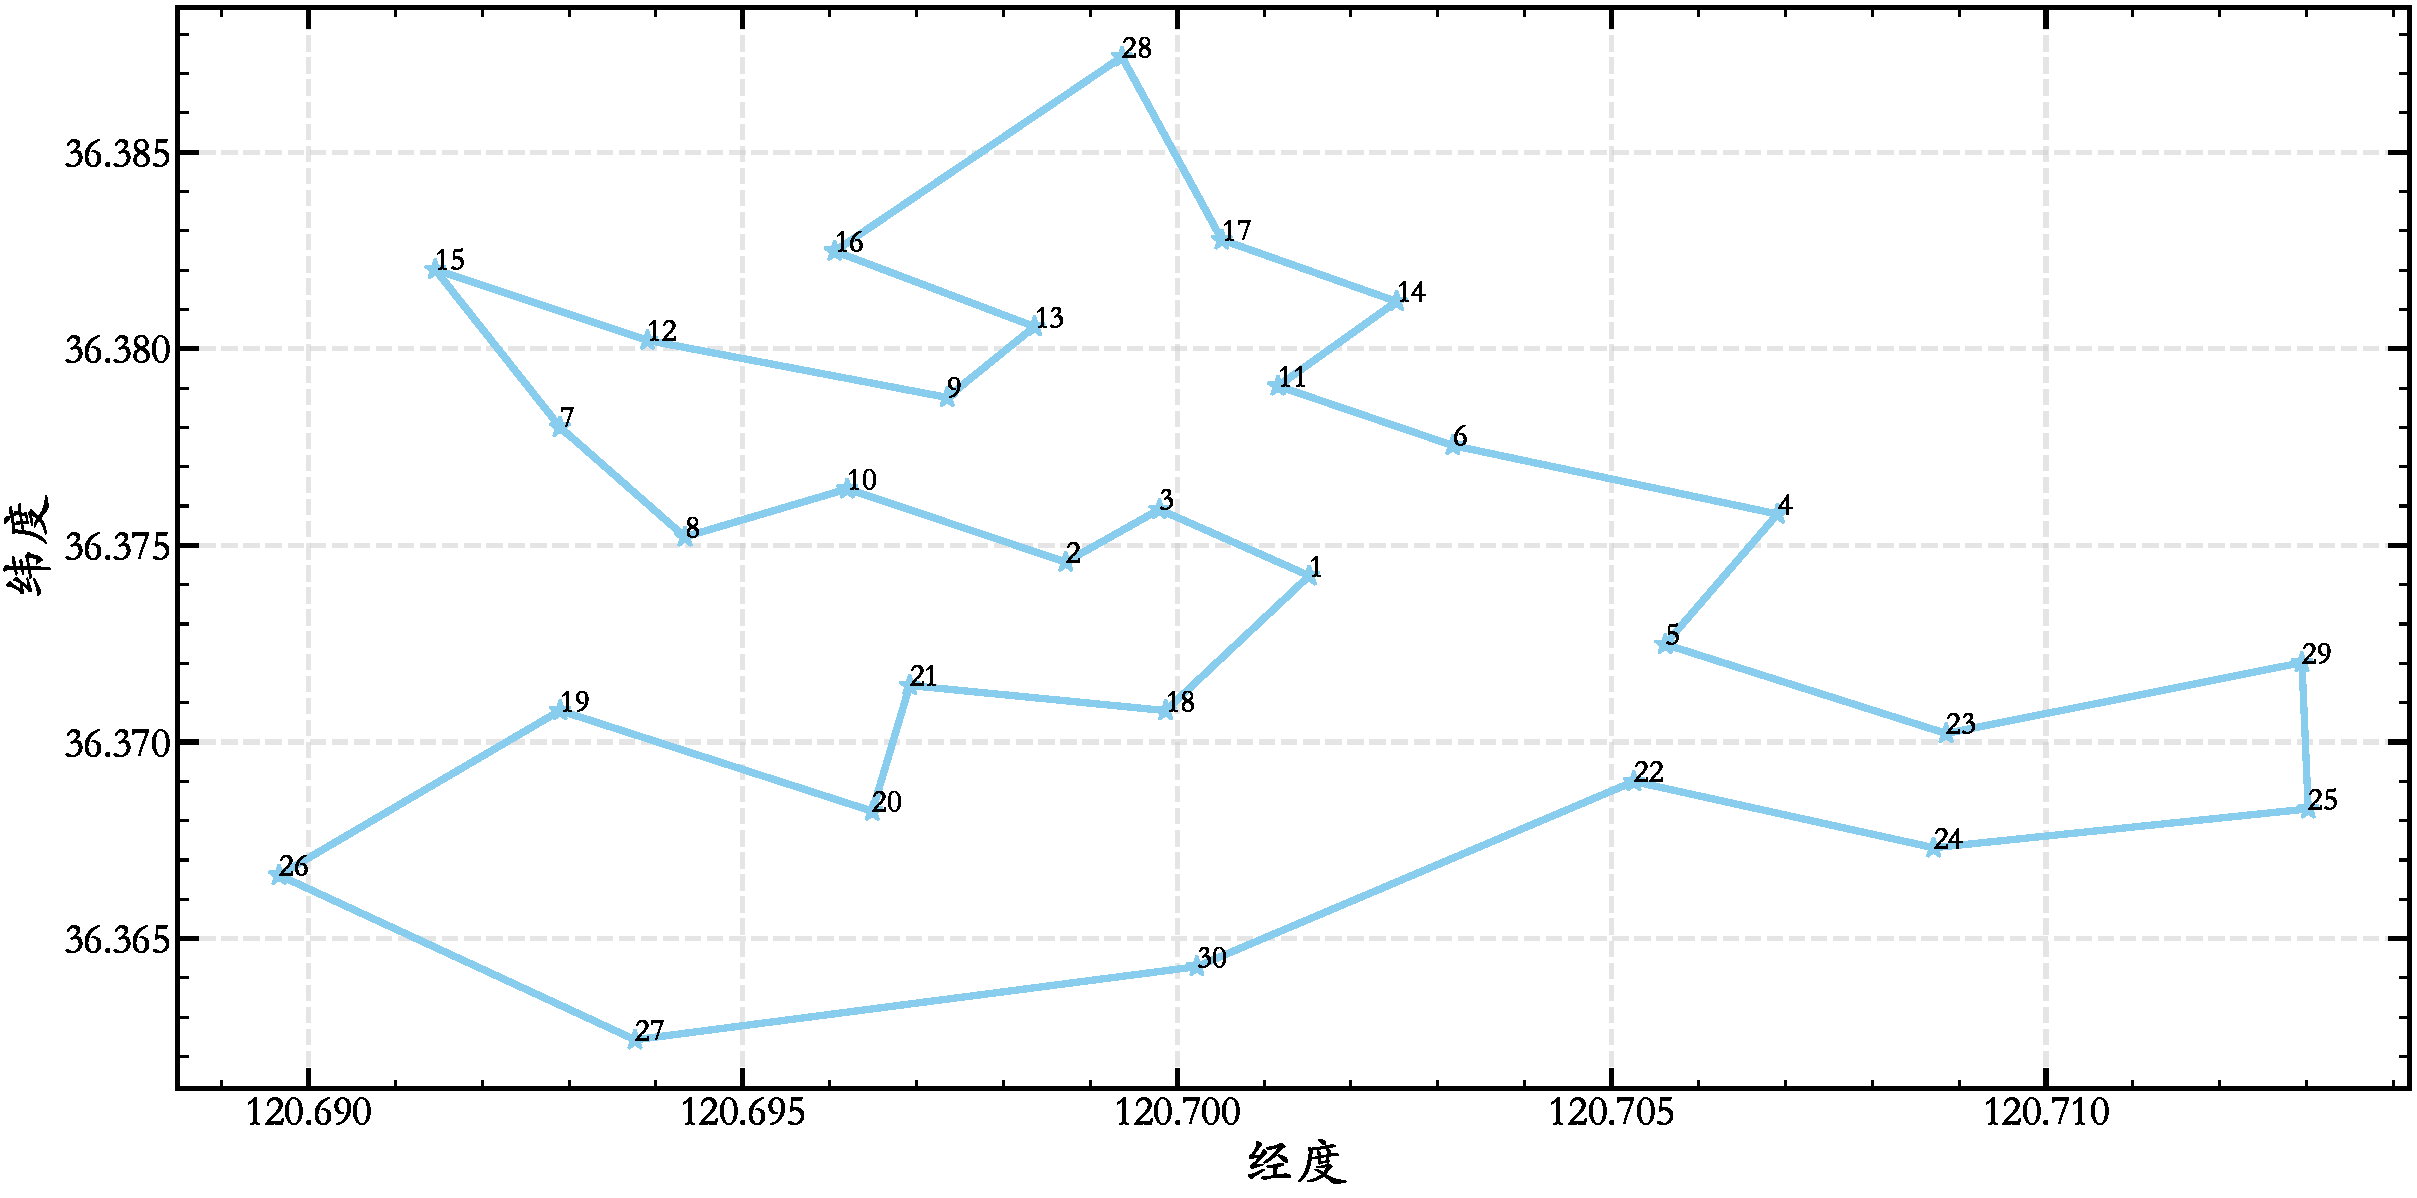
\includegraphics[width=0.6\textwidth]{lujing}
    \caption{路线图}
    \label{fig:road}
\end{figure}








\section{问题二:无线传感系统维稳的非线性规划模型}
\subsection{模型的建立}
根据图\ref{fig:road}的行驶路径、无线传感网络的充电策略以及查询到的相关资料,并且合理考虑现实情况,假定移动充电器充电速率为$r=1$、移动充电器移动速度为$v=5(m/s)$,供电器最小电池容量$f=50(mA)$。\par
值得一提的是,我们将附件二中29个节点的消耗速率单位转换为$(mA/s)$并记为$p_1,\cdots,p_{29}$以便之后的求解。
同时将问题一中求解得到的节点路径重排序并记录距离,例如从数据中心出发第一个到达的节点距离记为$s_1$,以此类推得到$s_1\cdots s_{30}$,最后再将单位转换为$(m)$。
\paragraph{决策变量}将各传感器最大容量设为$C_i$;在某一充电周期,将移动充电器到达各传感器时传感器剩余电量$b_{\text{剩}i}$;将移动充电器离开某一传感器时该传感器的电量设为$b_{\text{离}i}$。其中$i=1,\cdots,29$。

\paragraph{目标函数}题目要求每个传感器的电池的最大容量应至少是多大才能保证整个系统一直正常运行,所以我们的目标是保持无线传感系统稳定的情况下使每个传感器电池最大容量尽量小,即有:
\begin{gather*}
\min F=\sum_{i=1}^{29}C_i
\end{gather*}\par
综上,可以得到等式:
\begin{enumerate}[itemsep=0pt,parsep=0pt,label=(\arabic*)]
\item 各传感器充电时间为移动充电器从到达至离开期间克服耗电量的时长:
\begin{gather*}
t_{\text{充}i}=\frac{b_{\text{离}i}-b_{\text{剩}i}}{r-p_i}\\
\text{其中}i=1,2,\cdots,29
\end{gather*}
\item 所以我们自然可以得到各传感器最大充电时间即每周期各传感器在无线充电小车到达时电量为最低电池容量f,并且无线充电小车每次充电都将传感器电量充满:
\begin{gather*}
t_{\bm{max}i}=\frac{C_i-f}{r-p_i}\\
\text{其中}i=1,2,\cdots,29
\end{gather*}
\item 第i个节点和第i+1个节点(第1个和第31个节点都表示数据中心)之间移动时间:
\begin{gather*}
t_{i,i+1}=\frac{10^3\times s_i}{v}\\
\text{其中}i=1,2,\cdots,30
\end{gather*}

\item 一个充电周期总时长:
\begin{gather}
T=\sum_{i=1}^{29}t_{\text{充}i}+\sum_{i=1}^{30}t_{i,i+1}
\end{gather}
\end{enumerate}
\paragraph{约束条件}保证每个传感器从此次移动充电车离开到下次移动充电车到来期间(排除自身充电时长)电量保持在最低电量界限以上,所以有:
\begin{gather}
\label{ys1}
C_i-P_i\times(T-\frac{C_i-f}{r-p_i})\ge f\\
\text{其中}i=1,2,\cdots,29\notag
\end{gather}

事实上,我们可以得到:
\begin{theorem}
若各传感器最大充电时长满足约束时能使无线传感系统维稳,则任一周期下各传感器满足约束时的任意耗电情况及充电车充电情况都能使系统维稳
\end{theorem}
\begin{proof}
\begin{gather*}
\text{显然:}t_{\bm{max}i}\ge t_{\text{充}i}\\
\text{所以有:}T_{max}=\sum_{i=1}^{29}t_{\bm{max}i}+\sum_{i=1}^{30}t_{i,i+1}\ge T\\
\text{即得到:}C_i-P_i\times(T_{max}-\frac{C_i-f}{r-p_i})\ge C_i-P_i\times(T-\frac{C_i-f}{r-p_i})\ge f
\end{gather*}
\rightline{证毕}
\end{proof}
由定理1,可以将约束条件式(\ref{ys1})更新:
\paragraph{更新后约束条件}
\begin{gather}
C_i-P_i\times(T_{max}-\frac{C_i-f}{r-p_i})\ge f\\
\text{其中}i=1,2,\cdots,29\notag
\end{gather}
综上,建立无线传感系统维稳的非线性规划模型:
\begin{gather}
\min F=\sum_{i=1}^{29}C_i\notag\\
\begin{cases}
t_{\bm{max}i}=\frac{C_i-f}{r-p_i}\\
t_{i,i+1}=\frac{10^3\times s_i}{v}, \quad i=1,2,\cdots,30\\
T_{max}=\sum_{i=1}^{29}t_{\bm{max}i}+\sum_{i=1}^{30}t_{i,i+1}\\
C_i-P_i\times(T_{max}-\frac{C_i-f}{r-p_i})\ge f,\quad i=1,2,\cdots,29\\
\end{cases}
\end{gather}
\subsection{结果及参数分析}
假定充电速率r、最低电池容量f、行驶速度v后,求得各传感器最大电池容量如表\ref{tab:b1}。
\begin{table}[!h]
  \centering
  \caption{单车最大电池容量对应表}
    \begin{tabular}{rrrrrr}
	\toprule[1.5pt]
    1     & 2     & 3     & 4     & 5     & 6 \\
    53.59113 & 55.18373 & 52.99336 & 53.65753 & 52.39529 & 52.99336 \\
    7     & 8     & 9     & 10    & 11    & 12 \\
    54.25497 & 53.0598 & 52.99336 & 53.65753 & 52.99336 & 54.91845 \\
    13    & 14    & 15    & 16    & 17    & 18 \\
    54.32134 & 52.99336 & 52.52822 & 52.99336 & 53.65753 & 54.98477 \\
    19    & 20    & 21    & 22    & 23    & 24 \\
    53.65753 & 52.99336 & 52.32882 & 53.65753 & 54.98477 & 52.32882 \\
    25    & 26    & 27    & 28    & 29    &  \\
    53.65753 & 52.86048 & 52.39529 & 54.25497 & 53.59113 &  \\
    \bottomrule[1.5pt]
    \end{tabular}%
  \label{tab:b1}%
\end{table}%
计算表\ref{tab:b1}中最大最小差,与平均值相除得到的值为0.0546,即此类型电池容量的差异为5.46\%,由于电池容量通常存在5\%-10\%的差异\upcite{zhihu},因而符合实际情况,说明此模型良好。




\section{问题三:多台移动充电车的VRP模型}
\subsection{模型建立}
四台移动充电车同时从数据中心出发,题目要求规划移动充电器的充电路线以最小化所有移动充电器在路上的总的能量消耗。显而易见,这是一个典型的车辆路线(VRP)问题。\par
VRP问题最早是由Dantzig和Ramser于1959年首次提出,它是指一定数量的客户,各自有不同数量的货物需求,配送中心向客户提供货物,由一个车队负责分送货物,组织适当的行车路线,目标是使得客户的需求得到满足,并能在一定的约束下,达到诸如路程最短、成本最小、耗费时间最少等目的\upcite{toth2002vehicle}。旅行商问题是VRP的一个特例,所以VRP同样也是NP难问题。\par
与第一问类似,我们建立如下的VRP的整数规划模型
\begin{gather}
 \min \sum_{k \in K} \sum_{a \in A} c_{a} x_{a}^{k}\label{mb} \\
\begin{cases}
\label{yys}
\sum_{k \in K} \sum_{a \in \delta^{-}(i)} x_{a}^{k}=1, \quad \forall i \in N \\
\sum_{a \in \delta^{+}(i)} x_{a}^{k}=\sum_{a \in \delta^{-}(i)} x_{a}^{k}, \forall i \in N, \forall k \in K \\
\sum_{a \in \delta^{+}(o)} x_{a}^{k}=1, \forall k \in K \\
\sum_{a \in \delta^{-}(d)} x_{a}^{k}=1, \forall k \in K \\
\sum_{a \in \delta^{+}(S)} x_{a}^{k} \geq 1 \forall k \in K, \forall S \subset N \\
\text{决策变量}x_{a}^{k} \in\{0,1\}, \forall k \in K, \forall a \in A\\
\end{cases}\\
N:\text{传感器集合;}A:\text{路径集合:}K:\text{移动充电车集合}\notag\\
{o,d}\text{:数据中心}\notag\\
\delta^+(i)\text{代表所有从点i出发的弧}\notag\\
\delta^-(i)\text{代表所有进入点i的弧}\notag\\
\delta^+(S):\{(i,j)| (i,j)\in A,i\in S, j\notin S\}\text{(S是某点集)}\notag
\end{gather}\par
式(\ref{mb})表示目标函数即路径最短。(\ref{yys})中第一式表示每个传感器必须得到充电;第二式表示每个节点入流等于出流;第三、四式表示移动充电车必须从数据中心出发回到数据中心;第五式表示消除子回路,在求解中可采用问题一中第三个约束条件采取的办法即MTZ方法;第六式为决策变量。\par
接下来,将四台移动充电车的路径依次代入问题二中即维稳非线性规划模型,得到结果。
\subsection{结果及参数分析}
利用Gurobi求得四车行驶路径如图\ref{fig:4car}
\begin{figure}[!h]
    \centering
    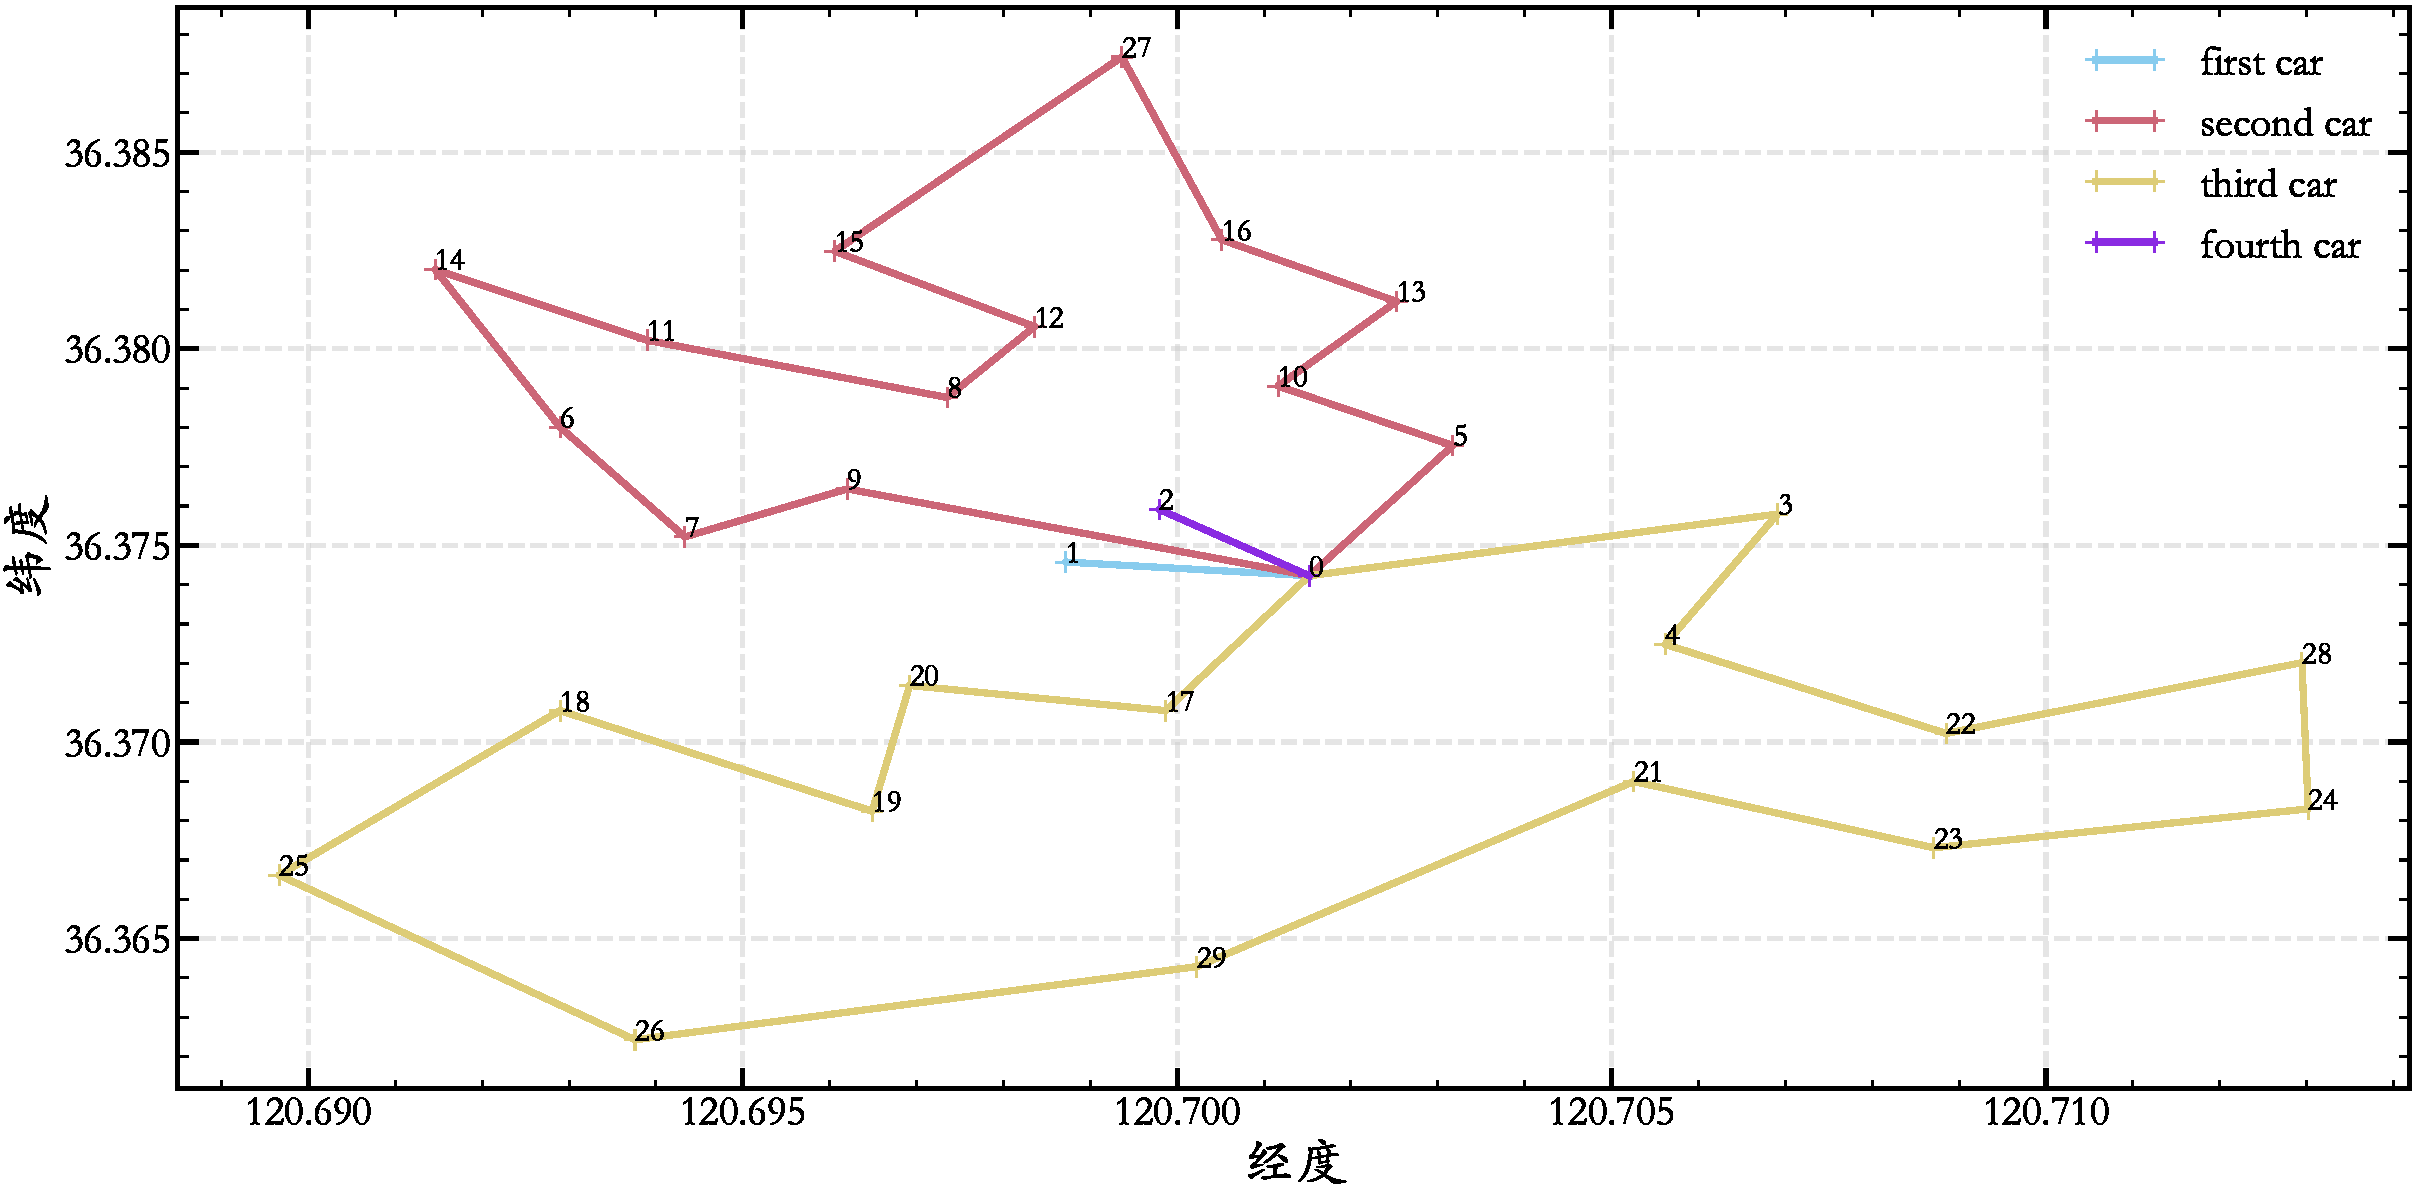
\includegraphics[width=0.6\textwidth]{4car}
    \caption{四车行驶路径}
    \label{fig:4car}
\end{figure}




沿用问题二所设参数,得到各传感器最大电池容量如表\ref{tab:b2}。
\begin{table}[!h]
  \centering
  \caption{四车最大电池容量对应表}
    \begin{tabular}{rrrrrr}
    \toprule[1.5pt]
    1     & 2     & 3     & 4     & 5     & 6 \\
    50.15232 & 50.21042 & 51.73167 & 52.1159 & 51.02212 & 51.27733 \\
    7     & 8     & 9     & 10    & 11    & 12 \\
    51.81569 & 51.30568 & 51.27733 & 51.56075 & 51.27733 & 52.09881 \\
    13    & 14    & 15    & 16    & 17    & 18 \\
    51.84401 & 51.27733 & 51.07885 & 51.27733 & 52.1159 & 52.88371 \\
    19    & 20    & 21    & 22    & 23    & 24 \\
    52.1159 & 51.73167 & 51.34723 & 52.1159 & 52.88371 & 51.34723 \\
    25    & 26    & 27    & 28    & 29    &  \\
    52.1159 & 51.6548 & 51.02212 & 52.46152 & 52.07748 &  \\
    \bottomrule[1.5pt]
    \end{tabular}%
  \label{tab:b2}%
\end{table}%
同样计算电池容量差异,结果为5.29\%,说明模型良好。


\section{模型的评价}
\subsection{模型优点}
\begin{itemize}
\item 运用Matlab的Gurobi加速器求解整数规划问题,在保障结果正确的同时,具有较快的计算速度;
\item 对模拟退火算法和遗传算法进行改进,运行结果兼具速度与精度;
\item 对模型结果可视化,直观,便于理解和分析;
\end{itemize}

\subsection{模型缺点}
\begin{itemize}
\item 第三题得出的规划路径为近似最优路径,并不是精确解,存在一定的偏差;
\item 基于假设得出的结果在某种程度上限制了模型的普适性和推广能力。
\end{itemize}
		
		

\bibliography{book.bib}
\newpage%附录新起一页
\begin{appendices}
\section{支撑材料}


	
\section{模拟退火代码}
\begin{matlab}
clc, clear, close all
sj=xlsread('data.xlsx');
d1=sj(1,:);%出发地、目的地经纬度
sj=sj(2:end,:);
xy=[d1;sj;d1];
amount=size(xy,1);
sj=xy*pi/180; %角度化成弧度
dist_matrix=zeros(amount); %距离矩阵d初始化
for i=1:amount-1
    for j=i+1:amount
        dist_matrix(i,j)=6370*acos(cos(sj(i,1)-sj(j,1))*cos(sj(i,2))*...
            cos(sj(j,2))+sin(sj(i,2))*sin(sj(j,2)));
    end
end
dist_matrix=dist_matrix+dist_matrix';
sol_new=[];E_current=inf; %巡航路径及长度初始化
for j=1:1000  %蒙特卡洛求较好的初始解
    path0=[1 1+randperm(amount-2),amount]; temp=0;
    for i=1:amount-1
        temp=temp+dist_matrix(path0(i),path0(i+1));
    end
    if temp<E_current
        sol_new=path0; E_current=temp;
    end
end
% sol_new是每次产生的新解;sol_current是当前解;sol_best是冷却中的最好解;
E_current = inf;E_best = inf; 
% E_current是当前解对应的回路距离;
% E_new是新解的回路距离;
% E_best是最优解的
sol_current = sol_new; sol_best = sol_new;
a = 0.99;% 温度衰减函数的参数
t0 = 100;%初始温度
tf = 0.1;%最低温
t = t0;
Markov_length = 10000;	% Markov链长度
pSwap=0.2;                          %选择交换结构的概率
pReversion=0.3;                     %选择逆转结构的概率
pInsertion=1-pSwap-pReversion;      %选择插入结构的概率
while t>=tf
    for r=1:Markov_length
        sol_new=Neighbor(sol_new,pSwap,pReversion,pInsertion);
        % 计算目标函数值
        E_new = 0;
        for i = 1 : (amount-1)
            E_new = E_new + ...
                dist_matrix(sol_new(i),sol_new(i+1));
        end
        % 再算上从最后一个城市到第一个城市的距离
        E_new = E_new + ...
            dist_matrix(sol_new(amount),sol_new(1));
        
        if E_new < E_current
            E_current = E_new;
            sol_current = sol_new;
            if E_new < E_best
                % 把冷却过程中最好的解保存下来
                E_best = E_new;
                sol_best = sol_new;
            end
        else
            % 若新解的目标函数值小于当前解的,
            % 则仅以一定概率接受新解
            if rand < exp(-(E_new-E_current)./t)
                E_current = E_new;
                sol_current = sol_new;
            else
                sol_new = sol_current;
            end
        end
    end
    t=t.*a;		% 控制参数t(温度)减少为原来的a倍
end
disp('最优解为:')
disp(sol_best)
disp('最短距离:')
disp(E_best)
xx=xy(sol_best,1); yy=xy(sol_best,2);
plot(xx,yy,'-*') %画出巡航路径
\end{matlab}
\section{遗传算法代码}
\begin{matlab}
clc,clear, close all
sj=xlsread('data.xlsx');
d1=sj(1,1:2);%出发地、目的地经纬度
sj=sj(2:end,1:2);
xy=[d1;sj;d1]; sj=xy*pi/180;  %单位化成弧度
amount=size(xy,1);
d=zeros(amount); %距离矩阵d的初始值
for i=1:amount-1
    for j=i+1:amount
        d(i,j)=6370*acos(cos(sj(i,1)-sj(j,1))*cos(sj(i,2))*...
            cos(sj(j,2))+sin(sj(i,2))*sin(sj(j,2)));
    end
end
d=d+d'; w=50; g=amount-2; %w为种群的个数,g为进化的代数
for k=1:w  %通过改良圈算法选取初始种群
    c=randperm(amount-2); %产生1,...,amount-2的一个全排列  
    c1=[1,c+1,amount]; %生成初始解
    for t=1:amount %该层循环是修改圈 
        flag=0; %修改圈退出标志
        for m=1:amount-2
            for n=m+2:amount-1
                if d(c1(m),c1(n))+d(c1(m+1),c1(n+1))<...
                        d(c1(m),c1(m+1))+d(c1(n),c1(n+1))
                    c1(m+1:n)=c1(n:-1:m+1);  flag=1; %修改圈
                end
            end
        end
        if flag==0
            J(k,c1)=1:amount; break %记录下较好的一组解并退出当前层循环
        end
    end
end
J(:,1)=0; J=J/amount; %把整数序列转换成[0,1]区间上实数即染色体编码
for k=1:g  %该层循环进行遗传算法的操作 
    A=J; %交配产生子代A的初始染色体
    c=randperm(w); %产生下面交叉操作的染色体对 
    for i=1:2:w  
        F=2+floor(amount-2*rand(1)); %产生交叉操作的地址
        temp=A(c(i),[F:amount]); %中间变量的保存值
        A(c(i),[F:amount])=A(c(i+1),[F:amount]); %交叉操作
        A(c(i+1),F:amount)=temp;  
    end
    by=[];  %为了防止下面产生空地址,这里先初始化
    while ~~isempty(by)
        by=find(rand(1,w)<0.1); %产生变异操作的地址
    end
    B=A(by,:); %产生变异操作的初始染色体
    for j=1:length(by)
        bw=sort(2+floor((amount-2)*rand(1,3)));  %产生变异操作的3个地址
        %交换位置
        B(j,:)=B(j,[1:bw(1)-1,bw(2)+1:bw(3),bw(1):bw(2),bw(3)+1:amount]); 
    end
    G=[J;A;B]; %父代和子代种群合在一起
    [SG,ind1]=sort(G,2); %把染色体翻译成1,...,amount的序列ind1
    num=size(G,1); long=zeros(1,num); %路径长度的初始值
    for j=1:num
        for i=1:amount-1
            long(j)=long(j)+d(ind1(j,i),ind1(j,i+1)); %计算每条路径长度
        end
    end
    [slong,ind2]=sort(long); %对路径长度按照从小到大排序
    J=G(ind2(1:w),:); %精选前w个较短的路径对应的染色体
    for m=1:floor(num*0.3)
        [sn,en]=SA(G(ind2(m),:));
        if en<slong(m)
            J(m)=sn;
        end
    end
end
path=ind1(ind2(1),:), flong=slong(1)  %解的路径及路径长度
xx=xy(path,1);yy=xy(path,2);
plot(xx,yy,'-o') %画出路径
\end{matlab}
\begin{matlab}
function [sol_best,E_best]=SA(sol_new)
sj=xlsread('data.xlsx');
d1=sj(1,1:2);%出发地、目的地经纬度
sj=sj(2:end,1:2);
xy=[d1;sj;d1];
num=size(xy,1);
sj=xy*pi/180; %角度化成弧度
d=zeros(num); %距离矩阵d初始化
for i=1:num-1
    for j=i+1:num
        d(i,j)=6370*acos(cos(sj(i,1)-sj(j,1))*cos(sj(i,2))*...
            cos(sj(j,2))+sin(sj(i,2))*sin(sj(j,2)));
    end
end
d=d+d';
amount=size(sol_new,2);
% sol_new是每次产生的新解;sol_current是当前解;sol_best是冷却中的最好解;
E_current = inf;E_best = inf; 
% E_current是当前解对应的回路距离;
% E_new是新解的回路距离;
% E_best是最优解的
sol_current = sol_new; sol_best = sol_new;
a = 0.99;% 温度衰减函数的参数
t0 = 100;%初始温度
tf = 99;%最低温
t = t0;
Markov_length = 10;	% Markov链长度
pSwap=0.2;                          %选择交换结构的概率
pReversion=0.3;                     %选择逆转结构的概率
pInsertion=1-pSwap-pReversion;      %选择插入结构的概率
while t>=tf
    for r=1:Markov_length
        sol_new=Neighbor(sol_new,pSwap,pReversion,pInsertion);
        % 计算目标函数值
        E_new = 0;
        [~,ind1]=sort(sol_new,2);
        for i = 1:amount-1
        E_new = E_new+d(ind1(i),ind1(i+1));
        end
        if E_new < E_current
            E_current = E_new;
            sol_current = sol_new;
            if E_new < E_best
                % 把冷却过程中最好的解保存下来
                E_best = E_new;
                sol_best = sol_new;
            end
        else
            % 若新解的目标函数值小于当前解的,
            % 则仅以一定概率接受新解
            if rand < exp(-(E_new-E_current)./t)
                E_current = E_new;
                sol_current = sol_new;
            else
                sol_new = sol_current;
            end
        end
    end
    t=t.*a;		% 控制参数t(温度)减少为原来的a倍
end
\end{matlab}
\section{问题1的0-1整数规划代码}
\begin{matlab}
clc, clear, close all
sj0=xlsread('C题附件1.xlsx');
x=sj0(2:30,1); x=x(:);
y=sj0(2:30,2); y=y(:);
sj=[x y]; d1=sj0(1,:); 
xy=[d1;sj;d1];
sj=xy*pi/180; %角度化成弧度
d=zeros(31); %距离矩阵d初始化
for i=1:30
   for j=i+1:31
       d(i,j)=6370*acos(cos(sj(i,1)-sj(j,1))*cos(sj(i,2))*cos(sj(j,2))+sin(sj(i,2))*sin(sj(j,2)));
   end
end
d=d+d';
for i = 1:31
    d(i,i)=10000; 
end
n=31;
x=binvar(31,31,'full');
u=intvar(31,1);
f=sum(sum(d.*x));
F=[];
F=[F;sum(x,2)==ones(n,1)];
F=[F;sum(x,1)'==ones(n,1)];
F=[F;u(1)==1;u(31)==31];
for i=2:n-1
    F=[F;2 <=u(i)<= n-1];
end
for i=1:n
    for j=2:n
        F=[F;u(i)-u(j)+n*x(i,j)<=n-1];
    end
end
ops=sdpsettings('solver','gurobi');
sol=solvesdp(F,f,ops);
f=double(f);
u=double(u);
x=double(x);
%%
a=[1:1:31]';
u=[a,u];
sort=sortrows(u,2);
path=sort(:,1);	
\end{matlab}
	
\section{问题2的非线性规划代码}	
\begin{matlab}
clc, clear, close all
sj0=xlsread('C题附件2.xlsx');
x=sj0(2:30,1); x=x(:);
y=sj0(2:30,2); y=y(:);
p=sj0(2:30,3); p=p(:)./3600;
sj=[x y]; d1=sj0(1,1:2); 
xy=[d1;sj;d1];
sj=xy*pi/180; %角度化成弧度
d=zeros(31); %距离矩阵d初始化
for i=1:30
   for j=i+1:31
       d(i,j)=6370*acos(cos(sj(i,1)-sj(j,1))*cos(sj(i,2))*cos(sj(j,2))+sin(sj(i,2))*sin(sj(j,2)));
   end
end
d=d+d';
path=[1,18,21,20,19,26,27,30,22,24,25,29,23,5,4,6,11,14,17,28,16,13,9,12,15,7,8,10,2,3,31];%问题1所求得路径
s=[];
for i=1:30
    s(i)=d(path(i),path(i+1));
end
c=sdpvar(29,1);
a=50;
v=5;
r=1;
f=sum(c);
F=[];
zz=0;
for i=1:29
    zz=zz+(c(i)-a)./(r-p(i));
end
for i=1:29
    F=[F;c(i)-p(i)*(sum((1000*s)./v)+zz-(c(i)-a)./(r-p(i)))>=a];
end
ops=sdpsettings('solver','fmincon','debug',0.5);
sol=optimize(F,f,ops);
a=double(a);
v=double(v);
r=double(r);
c=double(c);
cy=(max(c)-min(c))/min(c);
f=double(c);
\end{matlab}
	
\section{问题三规划代码}
\begin{matlab}
clear
clc
vNum=4;  %车数量
cusNum=30; %总节点数量
data=xlsread('C题附件1.xlsx');
x=data(:,1);y=data(:,2);
axis=[x y]; %城市坐标                                              
Dij=xlsread('data.xls');
%% 决策变量
Xijk=binvar(cusNum,cusNum,vNum,'full');%i、j节点之间是否由第k辆车进行配送
Yik=binvar(cusNum,vNum,'full'); %k辆车是否经过i节点
u=intvar(cusNum,1);
%% 目标函数
obj=0;
for i=1:cusNum
    for j=1:cusNum
        for k=1:vNum
            obj=obj+Dij(i,j)*Xijk(i,j,k);
        end
    end
end
f=obj;
%% 约束条件
F=[];
for i=2:cusNum
    F=[F;sum(Yik(i,:))==1]; %每个需求点i都会被一辆车经过
end

for i=1
    F=[F;sum(Yik(i,:))==vNum];%配送中心则会被所有用到的小车经过
end
for i=1:cusNum
    for j=1:cusNum
        for k=1:vNum
            if i==j
                F=[F;Xijk(i,j,k)==0];           %不可能存在从该点出发又回到该点的情况
            end
        end
    end
end

for i=1:cusNum
    for k=1:vNum
        F=[F;sum(Xijk(i,:,k))==sum(Xijk(:,i,k))];%流量平衡
    end
end


for j=1:cusNum
    for k=1:vNum
        F=[F;sum(Xijk(:,j,k))==Yik(j,k)];%Xijk和Yik的关系
    end
end

for i=1:cusNum
    for k=1:vNum
        F=[F;sum(Xijk(i,:,k))==Yik(i,k)];%Xijk和Yik的关系
    end
end

F=[F;u(1)==0];
for i=2:cusNum
    F=[F;1 <=u(i)<= cusNum-1];
end

for k =1:vNum
    for i=1:cusNum
        for j=2:cusNum
            F=[F;u(i)-u(j)+cusNum*Xijk(i,j,k)<=cusNum-1];
        end
    end
end
%% 求解
ops = sdpsettings( 'solver','gurobi');
sol=solvesdp(F,f,ops);
f=double(f);
Xijk=double(Xijk);
Yik=double(Yik);
% Uik=double(Uik);
%% 画图
plot(axis(2:cusNum,1),axis(2:cusNum,2),'ro');hold on;
plot(axis(1,1),axis(1,2),'pm');hold on;
for i=1:cusNum
    for j=1:cusNum
        for k=1:vNum
            if Xijk(i,j,k)==1
                plot([axis(i,1),axis(j,1)],[axis(i,2),axis(j,2)],'-');
            end
        end
    end
end
for k=1:vNum
    [a,b]=find(Xijk(:,:,k));
    sqe=[a,b];
    sqe1=zeros(1,0);
    sqe1(1)=1;
    [a,b]=find(sqe(:,1)==1);
    for i=2:length(sqe)+1
        [a,b]=find(sqe(:,1)==sqe1(i-1));
        sqe1(i)=sqe(a,b+1);
    end
    disp(['车辆',num2str(k),'的路径如下:']);
    disp(sqe1)
end
\end{matlab}
	
	
	
	
	
\section{python绘图代码}
\begin{python}
#encoding=gb2312
import pandas as pd
import numpy as np
from numpy import array,r_,c_,arange,savetxt
import matplotlib.pyplot as plt
path=[1,18,21,20,19,26,27,30,22,24,25,29,23,5,4,6,11,14,17,28,16,13,9,12,15,7,8,10,2,3,1]
index=(np.array(path)-1).tolist()
plt.style.use('science')
data=pd.read_excel('C题附件1.xlsx')
x=data.iloc[:,1]
x=np.array(x).flatten()
y=data.iloc[:,2]
y=np.array(y).flatten()
xy=c_[x,y];d1=array([[120.701520187911,36.3742269854581]])
xy=r_[xy,d1];
longtitude=xy[index,0]; latitude=xy[index,1];
plt.xlabel('经度');plt.ylabel('纬度')
for i in range(len(longtitude)):
    plt.text(longtitude[i],latitude[i],path[i],fontsize=15)
plt.plot(longtitude,latitude,'-*',markersize=10,linewidth=3)
plt.show()
\end{python}
	

	
	
	
	
	
	

\end{appendices}

\end{document}